%----------------------------------------------------------------
% FEUILLE DE STYLE ENSG au format Latex
%Classe de document pour le thème Latex de l'ENSG
% v.1 sept. 2010, D Lercier : création
% v.2 sept. 2012, T Coupin : création fichier classe et modif.
% v.3 sept. 2016, J. Beilin, modification de la gestion de la biblio + modifs mineures 
%----------------------------------------------------------------

\documentclass{themeensg}
\usepackage{color}

%---Texte en filigranne---
\SetWatermarkText{\textsc{Brouillon}}
%pour l'enlever : \SetWatermarkText{}
\SetWatermarkText{}

% mise en page no-stress
\renewcommand{\familydefault}{\sfdefault}
%-------------------------

%---Mes packages à moi---
%\usepackage{}
%------------------------

%---Mes raccourcis---
\newcommand{\transpose}[1]{{}^t \! #1}
\newcommand{\ensg}{\textsc{Ensg}}

\renewcommand{\author}{Bob L'Éponge}

%--------------------

%---Paramètres du pdf---
    \hypersetup{
       backref=true,                           % Permet d'ajouter des liens dans
       pagebackref=true,                       % les bibliographies
       hyperindex=true,                        % Ajoute des liens dans les index.
       colorlinks=true,  %Colorise les liens : true pour version numérique, false pour version d'impression
       breaklinks=true,                        % Permet le retour à la ligne dans les liens trop longs.
       urlcolor= blue,                         % Couleur des hyperliens.
       linkcolor= blue,                       % Couleur des liens internes.
       bookmarks=true,                         % Créé des signets pour Acrobat.
       %bookmarksopen=true,                    % Si les signets Acrobat sont créés,
                                               % les afficher complètement.
       pdftitle={Thème ENSG},                 % Titre du document.
                                               % Informations apparaissant dans
       pdfauthor={\author},                      % dans les informations du document
       pdfsubject={Feuille de style ENSG}           % sous Acrobat.
    }

%-----------------------



%-------------------------------------------------------------

\setcounter{tocdepth}{1} %profondeur de la table des matières

\title{Feuille de style \LaTeX~de l'\ensg\\Documentation plus que rapide\\Version provisoire du \today~à \timenow}

\bibliography{latexppmd}

%
%-------------------------------------------------------------
% Début du document
%--------------------------------------------------------------
\begin{document}
%--------------------------------------------------------------
\begin{titlepage}
%Inclusion des labels des entreprises
%Pour un seul label (à gauche), mettre NULL pour les 3e et 4e argument
\enterprise 
{logos/logo_ensg}
{Ecole Nationale des Sciences Géographiques}
{logos/logo_entreprise}
{Nom de l'entreprise d'accueil}

%Inclusion du titre

\textit{{\color{red}Choisir les intitulés et responsables pédagogiques (p2) qui conviennent suivant votre cursus - ing3 ou MS PPMD-}}

\maketitle{{\color{red}Rapport de stage} ou {\color{magenta}Thèse Professionnelle}\\{\color{red}Cycle des Ingénieurs diplômés de l'ENSG 3\up{ème} année} ou {\color{magenta}Mastère spécialisé$\circledR$ Photogrammétrie, Positionnement, Mesure de Déformations}}{logos/logo_ensg}



\infos{\author}{Novembre 2017}
\end{titlepage}

%\begin{comment}
% ---Page du jury---
%---Page du jury---
%\newevenpage
\thispagestyle{plain}
\section*{Jury}
\vspace{0.5cm}

\textbf{Président de jury :} \\

Victor Coindet
Professeur de l'ENSG, Responsable du cycle TSI

\vspace{0.5cm}

\textbf{Commanditaire :} \\

M. Sebastien Connesson, COO de Galigeo

\vspace{0.5cm}

\textbf{Encadrement de stage :} \\ 

M. Jean-Michel Gaudin, Product Leader à Galigeo
M. Raimana Teina, Product Dev Leader à Galigeo

\vspace{0.5cm}

\textbf{Enseignant référent :} \\ 

M. Loic Landrieu, Chercheur MATIS / IGN, Professeur de l'ENSG

\vspace{0.5cm}

\textbf{Rapporteur expert :} \\ 

qui est rapporteur du mémoire ?

\vspace{0.5cm}

\textbf{Responsable pédagogique du cycle Ingénieur - TSI:} \\

Victor Coindet
Professeur de l'ENSG, Responsable du cycle TSI

\vspace{0.5cm}

\textbf{Gestion du stage :} \\ 

Delphine Genès, Relation entreprise de l'ENSG

\vspace{0.5cm}


\section*{Stage de fin d'étude du 2 mai 2022 au 28 Octobre 2022}
\vspace{0.3cm}
\textbf{Diffusion web :} $\boxtimes$ Internet \hspace{0.2cm}$\boxtimes$ Intranet Polytechnicum\hspace{0.2cm}
$\boxtimes$ Intranet ENSG\vspace{0.3cm}

\textbf{Situation du document :} 
\vspace{0.2cm}
\par
Rapport de stage de fin d'études présenté en fin de 3\up{ème} année du cycle des Ingénieurs
\vspace{0.3cm}


\newcounter{x}
\setcounter{x}{\getpagerefnumber{LastPage}-\getpagerefnumber{beginappendices}+1}

\textbf{Nombres de pages :} \getpagerefnumber{LastPage} pages dont \arabic{x} d'annexes
\vspace{0.3cm}

\textbf{Système hôte :} \LaTeX
\vspace{1cm}


\textbf{Modifications :} 
\begin{center}
\begin{tabular}{|c|c|c|>{\centering}p{6.5cm}|}
\hline 
EDITION & REVISION & DATE & PAGES MODIFIEES\tabularnewline
\hline
\hline 
1 & 0 & 09/2022 & Création\tabularnewline
\hline 

\end{tabular}
\end{center}
%------------------

%------------------------------------------------------------------------------
% Remerciements
\newevenpage
\chapter*{Remerciements}

Je remercie


%---Résumé (français)---
\begin{abstract}
\thispagestyle{empty}
	\vspace{1cm}

	Ceci est mon résumé bla bla bla
	
	\vspace{1.5cm}
	
	\textbf{Mots clés :} clés, clés, clés
\end{abstract}
%-----------------------


%---Résumé (anglais)---
%\selectlanguage{english}
\begin{abstract}
\thispagestyle{empty}
	\vspace{1cm}
	
	This is my abstract blah blah blah...
	
	\vspace{1.5cm}
	
	\textbf{Key words:} key, key, key
\end{abstract}
%----------------------

\selectlanguage{french}

%---Table des matières, des figures et des tableaux---
\newevenpage
\tableofcontents



\newevenpage
\chapter*{Glossaire et sigles utiles}
\addcontentsline{toc}{chapter}{Glossaire et sigles utiles}

  \begin{acronym}
  \acro{ENSG}{\'Ecole Nationale des Sciences Géographiques}
  \acro{GNSS}{Global Navigation Satellite Systems}
  \acro{GPS}{Global Positionning System}
  \end{acronym}


%---Introduction------------------------------------------------------------------
\newevenpage
\chapter*{Introduction}
  \addcontentsline{toc}{chapter}{Introduction}
  
  \vspace{1.5cm}
	J'introduis

%-------------------------------------------------------------------------------
%\end{comment}

\evenchapter[Galigeo \ensg]{Galigeo}

\section{Présentation de l'entreprise}

\subsection{Généralités}

Galigéo est une société parisienne spécialisée dans le géomarketing. Créée en 2001, elle propose aux entreprises d’améliorer l’efficacité de tous leurs métiers grâce à ses logiciels combinant expertise cartographique et modélisation prédictive. Grâce à ses logiciels visualisant, analysant et agissant directement sur les bases de données opérationnelles (applications métier, BI, CRM, …). Galigeo permet aux utilisateurs de se focaliser sur leur métier (distribution, marketing, sécurité, …).

Historiquement pionnier de la location Intelligence, Galigeo a poursuivi son développement ces dernières années en ajoutant la composante prédictive dans ses suites logiciels, composante basée sur les techniques innovantes de Machine Learning et d’Intelligence Artificielle.

En utilisant son expertise cartographique et de modélisation prédictive, Galigeo poursuit son développement en mettant à disposition de ses clients, des logiciels simples d’usage, à très forte valeur ajoutée métier.

De 2001 à 2006, Galigeo se consacre aux développements de solutions intelligentes en géodécisionnel pour faire de l'analytique avancée à partir de cartes géographiques. De 2006 à 2011, elle développe sa première solution logiciel, Galigeo Enterprise, qui permet par la suite, grâce à un nouveau pôle Conseil, de proposer des services spécifiques métier et adaptés à chaque client autour du géomarketing. A partir de cette date, Galigeo va voir sa croissance augmenter sur le marché international en s'associant à différents partenaires. A partir de 2017 et jusqu'à aujourd'hui, Galigeo a choisi d'ajouter à ses solutions une composante prédictive très demandée sur le marché.

L'entreprise compte aujourd'hui une cinquantaine de clients très divers, grandes enseignes commerciales, services publiques, industries, etc. Galigeo peut fournir des solutions logiciels standards pour permettre à n’importe quelle entreprise de générer des rapports de géomarketing en utilisant des données internes et des données générales fournies par Galigeo. Elle réalise également des projets plus spécifiques, propres à des besoins bien déterminés qui permettent alors à ses clients d’avoir une vraie valeur ajoutée et un géomarketing efficace.

% Image of the offices
\begin{figure}[H]
    \centering
    
\includegraphics[width=\linewidth]{images/logos/client.png}
    \caption{Exemple de clients Galigeo}
    \label{fig:clients}
\end{figure}

Les bureaux de l'entreprise sont situés au 87 avenue d'Italie dans le treizième arrondissement de Paris.

% Image of the offices
\begin{figure}[H]
    \centering
    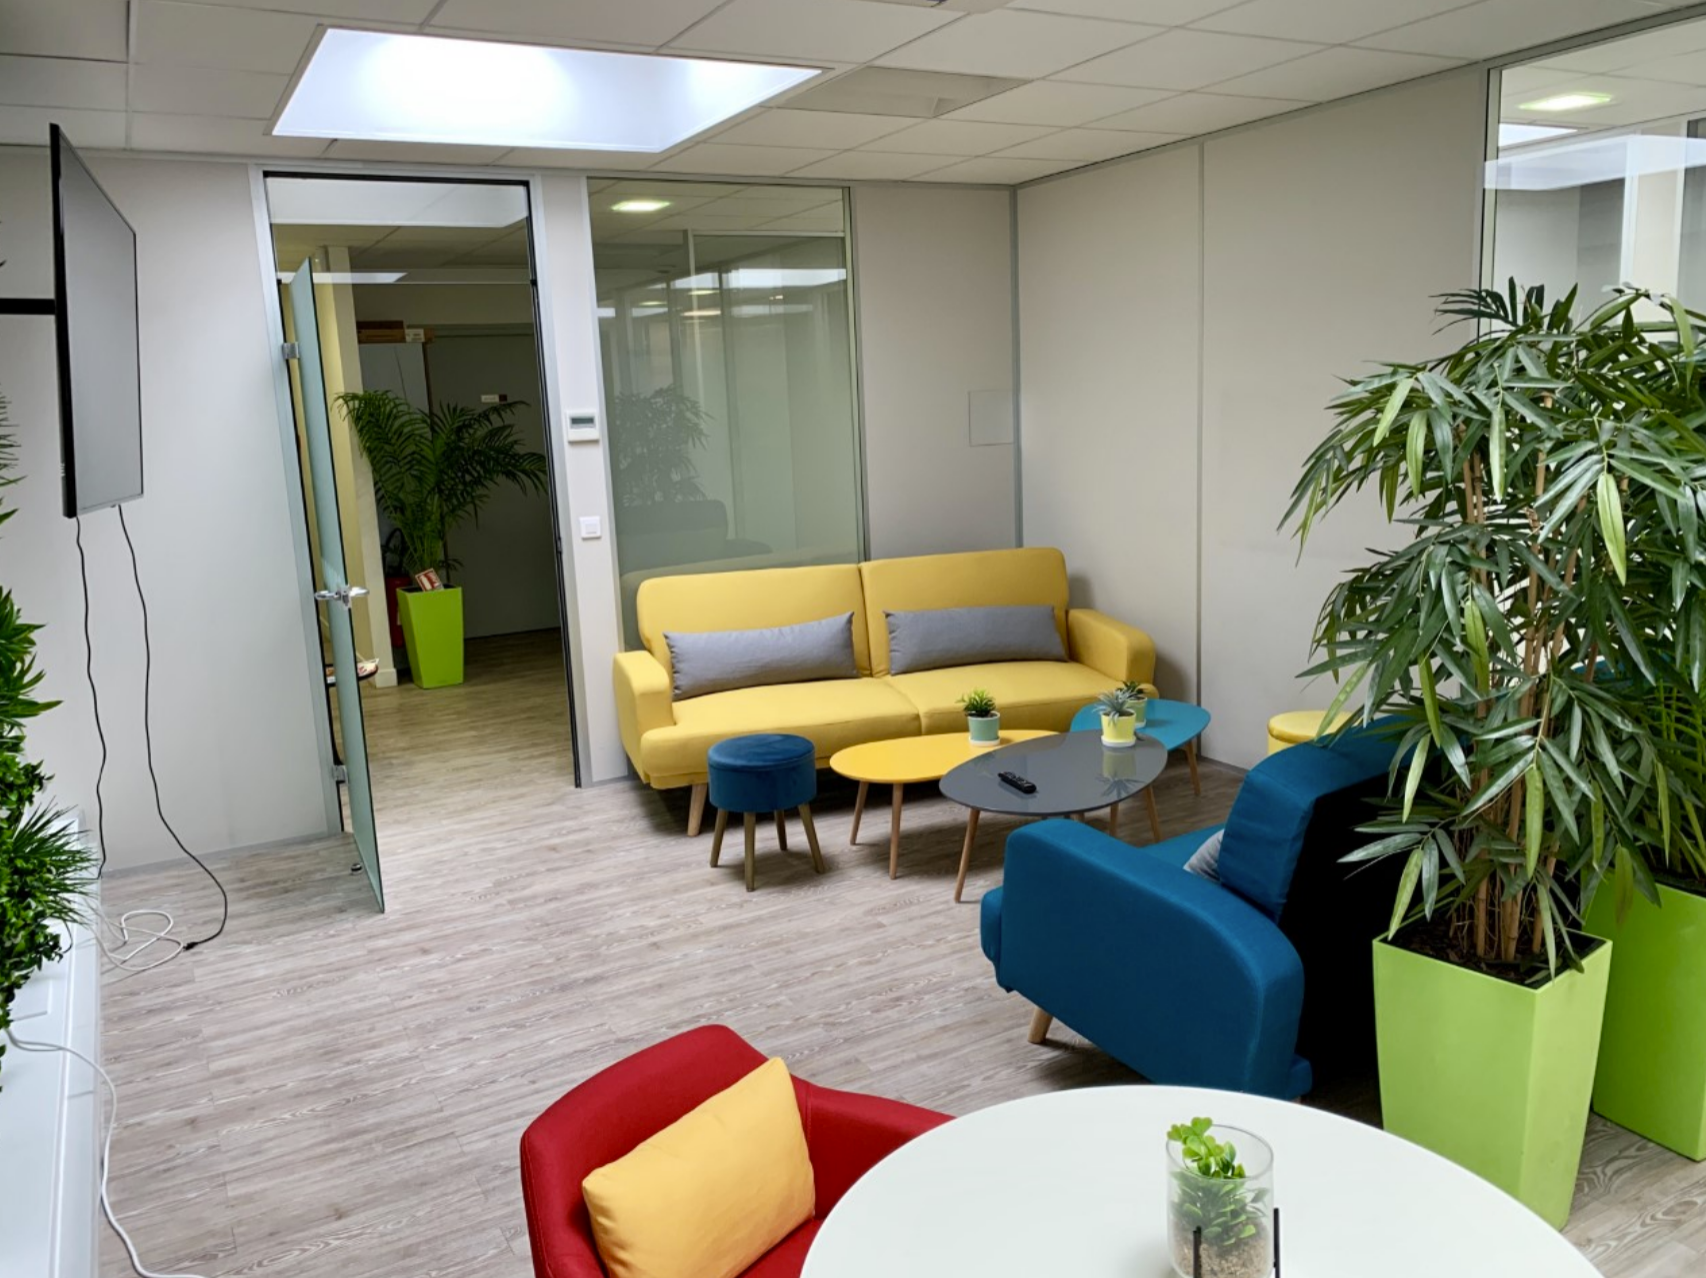
\includegraphics[width=12cm]{images/photos/bureaux_galigeo.png}
    \caption{Bureaux de Galigeo, 87 avenue d'Italie, 75013 Paris}
    \label{fig:offices}
\end{figure}


\subsection{Organisation interne}

Galigéo est composé actuellement d’une vingtaine d’employés répartis dans 5 pôles : Administratif, Commercial, Marketing, Comptabilité, Consulting et Recherche et Développement.

Le pôle administratif est le pôle qui s’occupe de la gestion du budget, du personnel et des missions à Galigeo.

Le pôle commercial gère les relations clients, il propose des offres à de nouveaux ou anciens clients, prospecte et cherche à faire grandir le cercle de clientèle de Galigeo.

Le pôle marketing imagine les produits, met en place les stratégies de pénétration du marché et réalise un catalogue de solutions que Galigeo peut fournir.

Le pôle comptabilité est responsable de la facturation des clients et la gestion interne des frais de personnels, des salaires, du matériel, etc.

Le pôle consulting est dédié à la réponse aux besoins techniques du client, il permet de rester proche du client. Il imagine les solutions retenues et les intègre dans les outils Galigeo mis à disposition pour l’entreprise.


Pour ma part, j’ai rejoint le pôle Recherche et Développement. L’équipe est composée de développeur, de testeurs, de designeurs, de data scientist, etc. Elle s’attache à améliorer les produits de Galigeo et à faire du support, de la maintenance et de l’innovation. Lorsqu’un consultant est en charge d’un projet pour un client, il s’appuie sur un ou plusieurs membres de l’équipe R\&D pour conseiller ou réaliser les tâches techniques.

\paragraph*{}

J’ai principalement travaillé avec Raimana Teina, Data Sientist chez Galigeo autour du grand projet actuel chez Galigeo « Prédiction de flux piéton » que je détaillerai dans la suite de ce rapport. Cependant j’ai également eu l’occasion de travailler sur des projets clients avec l’équipe consulting. 

% Image of the offices
\begin{figure}[H]
    \centering
    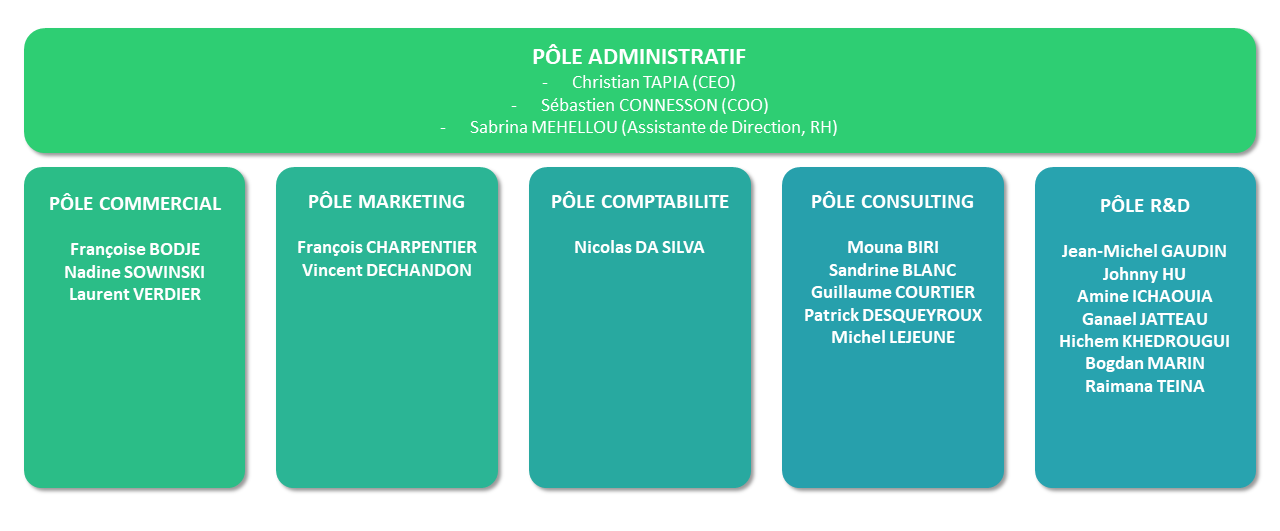
\includegraphics[width=\linewidth]{images/graphs/organigramme.png}
    \caption{Organigramme de Galigeo}
    \label{fig:organigrame}
\end{figure}


\section{Les objectifs de Galigeo}

\subsection{Les manques actuels}

Aujourd’hui, Galigeo cherche à mettre en avant des modèles prédictifs au service du géomarketing pour ses clients. Une mesure importante en géomarketing est l’estimation de flux piéton à un endroit donné et sur une période donnée. Jusqu’ici, Galigeo utilisait un service tiers afin d’obtenir une estimation de flux piéton. Cette solution de transition possède néanmoins de nombreux défauts. Tout d’abord Galigeo n’avait aucune visibilité sur les algorithmes utilisés pour faire cette estimation.

Il était alors difficile d’utiliser les résultats de cette estimation dans l’entraînement de nouveaux modèles de prédiction (estimation de chiffre d’affaires, estimation de parts de marchés, etc.). De plus, les coûts d’une telle solution restent élevés.

Il a donc été décidé de créer un modèle d’estimation de flux piéton propre à Galigeo sur lequel l’entreprise aurait accès à toutes les données d’entrées du modèle. Ainsi elle pourra modéliser d’autres variables essentielles au géomarketing plus facilement et avec une meilleure qualité. En effet, en connaissance des biais de notre modèle, ils seront plus faciles à corriger dans d’autres cas d’utilisation.

Galigeo souhaite également renforcer son équipe big data afin de mettre en valeur de grosses quantités de données brutes inexploitables en l’état. En recrutant de nouveaux data scientist, elle libèrera du temps à ses consultants et déchargera les équipes spécialisées dans la data actuellement en place.

\paragraph*{}

Après un entretien au printemps 2022 chez Galigeo et cette explication des manques et objectifs de l’entreprise à court terme, j’ai fait part de mon envie de réaliser un stage au sein de l’équipe R\&D. Ils ont retenu ma candidature et j’ai donc commencé mon stage de fin d’étude le 02 Mai 2022.


\subsection{Les objectifs du stage}

Durant ce stage j’avais donc comme première objectif de découvrir le géomarketing dans son ensemble. J’ai dû analyser et comprendre les cas d’usages métiers et me plonger dans le fonctionnement d’une équipe de développement logiciel.

J’avais également pour mission de concevoir et spécifier des solutions d’acquisition, de cleaning et de traitement des données. Comprendre le fonctionnement des produits Galigeo m’a permis de collecter et stocker la donnée de manière optimale afin de faciliter l’implémentation dans des bases de données.

J’avais également pour mission de développer des chaînes de collecte de la donnée en m’appuyant sur des méthodes de data engineering \footnote{Ingénierie des données}. Pour pouvoir par la suite utiliser au mieux la donnée dans des processus d’analyse et de traitement.

Pour la partie traitement de la donnée brute, mes objectifs étaient de développer des algorithmes et des traitements de la data grâce à des méthodes statistiques et de machine learning. Mon objectif était de transformer de la donnée brute inexploitable en une donnée pertinente pour le géomarketing des clients Galigeo.

\paragraph*{}

Mon objectif était également de m’intégrer aux équipes de Galigeo afin de mieux comprendre les objectifs de l’entreprise à long terme et les directions à prendre.


\subsection{Les objectifs à plus long terme}

Galigeo cherche aujourd’hui à implémenter de plus en plus de modèles prédictifs dans ses solutions. Pour cela, elle veut s’appuyer sur la big data et la data science qui permettent d’obtenir des résultats de qualité et qui intéressent aujourd’hui le marché du géodécisionnel.

Galigeo cherche donc à développer son équipe R\&D spécialisée dans la data afin de créer de nouveaux modèles compétitifs vis-à-vis des solutions concurrentes existantes et ainsi attirer de nouveaux clients et apporter des nouveautés aux plus anciens.

\paragraph*{}

Aujourd’hui ces modèles prédictifs permettent d’évaluer une variable à un endroit spécifique (footfall \footnote{Flux piéton}, chiffre d’affaires, cannibalisation, …). On peut alors comparer plusieurs localisations et déterminer laquelle est la plus intéressante pour une entreprise.

Il sera alors pertinent de s’intéresser à des modèles de recherche qui permettent de trouver directement la meilleure localisation pour une variable donnée.


\section{Organisation du stage}

\subsection{Planning}

Le planning complet de mon stage est disponible en annexe \ref{planning_gannt}. Il est détaillé sur la période Mai - Septembre 2022. La rédaction de ce rapport a eu lieu avant la définition des tâches d'octobre.

\subsection{Mes missions}

Ma mission principale à Galigeo était de réaliser des modèles prédictifs de variables utiles au géomarketing. L’estimation du flux piéton en une adresse a été ma principale mission. Cependant j’ai également passé quelques temps sur la modélisation de chiffres d’affaires pour une marque de produit culturel et électronique française. J’ai dû également modéliser la cannibalisation qu’entraînerait l’ouverture d’une enseigne proche d’une autre sur le territoire français.

\paragraph*{}

Ces deux missions mettaient en pratique mes compétences en Machine Learning acquises à l’ENSG. Je reviendrai sur ma mission sur le flux piéton dans la partie 2.2 de ce rapport. Pour la partie modélisation de chiffres d’affaires et d’estimation de cannibalisation, j’y reviendrai dans la partie 2.3.

\paragraph*{}

J’ai également réalisé d’autres plus petites missions pour Galigeo. J’ai eu la chance de travailler quelques jours sur un projet d’analyse de données et sur un projet de data engineering pour une compagnie internationale. Je détaillerai rapidement ces deux derniers projets dans la partie 2.4 de mon rapport.


\subsection{Relations internes et client}

Dans le pôle R\&D, le travail est organisé autour de la méthode Agile \footnote{Méthode de travail en équipe}. Un sprint \footnote{Rassemblement de tâches à executer dans un temps donné} dure environ 2 semaines et nous faisons un point tous les jours à 15h30 pour communiquer sur notre avancement et les difficultés rencontrés afin de pouvoir répondre rapidement aux besoins de chacun.

Je peux télétravailler 2 jours par semaine et cela fonctionne très bien car la plupart des réunions en présentiel sont également retransmises en visio-conférence. Galigeo utilise la suite Office 365 Professionnel ce qui permet d’organiser facilement le travail et les interactions.

\paragraph*{}

J’ai également travaillé sur des projets où j’échangeais uniquement avec le pôle consulting. Dans ce cas-là, nous avions des réunions quotidiennes également avec le consultant en question et une réunion hebdomadaire avec le client.




%\begin{comment}
%-------------------------------------------------------------------------------
\newevenpage
\chapter*{Conclusion}
  \addcontentsline{toc}{part}{Conclusion}
  \vspace{1.5cm}
Il est l'heure de conclure : bonne nuit !


%-------------------------------------------------------------------------------
% Insertion de la bibliographie
\newevenpage
%\printbibheading
\printbibliography[title={Bibliographie}]
\nocite{*}

\newevenpage
\listoffigures

\newevenpage
\listoftables
%----------------------------------------------------

\newevenpage
\begin{appendices} 
\label{beginappendices}
\annexe[Filtre de Kalman]{Filtre\newline de Kalman}
\label{annexekalman}
Contenu de l'annexe sur Kalman...

\annexe[Moindres carrés]{Moindres carrés}
\label{annexemc}
Contenu de l'annexe sur MC...

\end{appendices} 
%\end{comment}
\end{document}